\documentclass[11pt]{article}
\usepackage{geometry}                
\geometry{letterpaper}                 
\usepackage[parfill]{parskip}        
\usepackage{graphicx}
\usepackage{subfigure}
\usepackage{amssymb}
\usepackage{amssymb}
\usepackage{amsmath}
\usepackage{epstopdf}
\usepackage{verbatim}
\usepackage{float}
\usepackage{grffile}
\usepackage{fullpage}
\usepackage{enumerate}
\usepackage{hyperref}
\usepackage[utf8]{inputenc}
\usepackage{gensymb}
\usepackage[T1]{fontenc}
\usepackage[hang,small]{caption}
\DeclareGraphicsRule{.tif}{png}{.png}{`convert #1 `dirname #1`/`basename #1 .tif`.png}

\graphicspath{ {C:/Users/Nate/Documents/School/EECS351/Nates Discussion Material/Discussion 3} }
\usepackage{listings}
\usepackage{color}
\usepackage{textcomp}
\definecolor{listinggray}{gray}{0.9}
\definecolor{lbcolor}{rgb}{1,1,1}
\lstset{
	backgroundcolor=\color{lbcolor},
	tabsize=4,
	rulecolor=,
	language=matlab,
	basicstyle= \scriptsize,
	upquote=true,
	aboveskip={1.5\baselineskip},
	columns=fixed,
        	showstringspaces=false,
        	extendedchars=true,
        	breaklines=true,
        	prebreak = \raisebox{0ex}[0ex][0ex]{\ensuremath{\hookleftarrow}},
        	frame=single,
        	showtabs=false,
        	showspaces=false,
        	showstringspaces=false,
        	identifierstyle=\ttfamily,
        	keywordstyle=\color[rgb]{0,0,1},
        	commentstyle=\color[rgb]{0.133,0.545,0.133},
        	stringstyle=\color[rgb]{0.627,0.126,0.941},
}


\begin{document}

\section*{EECS351 Discussion 3 Solutions, 09/22/16}
Nate Sawicki \newline
Select problems by Mai Le and Kevin Moon

\section*{2 Problems}
\subsection*{Problem 1}
Vectors v1 and v2 are orthogonal and have unit length. So now we just show that the standard basis can be formed as a weighted sum of v1 and v2.

\vspace{4mm}
\emph{Solution:}
Lets show that v1 and v2 can express the standard/canonical basis vectors using a weighted sum:
\begin{center}
\[
B = 
\begin{bmatrix}
   v_1  \hspace{3mm}  v_2 
\end{bmatrix}
\]
\end{center}

\begin{center}
\[
B = 
\begin{bmatrix}
   3/\sqrt{10} \hspace{3mm}   1/\sqrt{10} \\
   1/\sqrt{10} \hspace{3mm}   -3/\sqrt{10}           
\end{bmatrix}
\]
\end{center}

\vspace{4mm}

Consider ($\sqrt{10}v_1$ - 3$\sqrt{10}v_2$)/10 =

\begin{center}
\[
B = 
\begin{bmatrix}
   0 \\
 1
\end{bmatrix}
\]
\end{center}


\vspace{4mm}

Consider (3$\sqrt{10}v_1$ + $\sqrt{10}v_2$)/10 =

\begin{center}
\[
B = 
\begin{bmatrix}
   1 \\
 0
\end{bmatrix}
\]
\end{center}

\vspace{5mm}

\subsection*{2.2 \hspace{3mm} Problem 2}
A = $B^{-1}$ since A is orthornormal, $B^{-1}$  = $B^{T}$  = B


\vspace{5mm}

\subsection*{2.3 and 2.4 \hspace{3mm} Problem 3 and 4}
Draw a line segment from A to C.

\begin{center}

\textbf{z} = 2*$v_1$ + $v_2$ = [2.21 -.32]$^{T}$

\end{center}

\vspace{5mm}

\subsection*{2.5 \hspace{3mm} Problem 5}
Solve for \textbf{z} analytically. Using Matlab to verify:

\begin{center}

\textbf{z} = B\textbf{x} = [2.21 -.32]$^{T}$



\end{center}


\vspace{5mm}

\subsection*{2.6 \hspace{3mm} Problem 6}
Since B is orthornomal and symmetric: 

\begin{center}

 $B^{-1}$  = $B^{T}$  = B



\end{center}

\vspace{5mm}
\begin{center}

 $B^{T}$z  = \textbf{x} = [2 1]${^T}$



\end{center}



\subsection*{3 Inner Product}
\begin{center}

||z||$^2$

\end{center}
\begin{center}

= ||x + y||$^2$

\end{center}
\begin{center}

= (x+y)(x+y)

\end{center}

\begin{center}

= $x^2 + 2xy + y^2$

\end{center}

\begin{center}

xy = 0 since x $\perp$ y

\end{center}

\begin{center}

= $x^2 + y^2$ = ||x||$^2$ + ||y||$^2$

\end{center}





\newpage

\begin{center}

\textbf{x} = x[n] = 
$
\begin{bmatrix}

x \\
y

\end{bmatrix}
$
\end{center}

\vspace{5mm}

\begin{center}
\[
B = 
\begin{bmatrix}
   b_1  \hspace{3mm}   b_3 \\
   b_2 \hspace{3mm}   b_4            
\end{bmatrix}
\]
\end{center}

Let $v_1$ = [$b_1$ $b_2$]$^T$, $v_2$ = [$b_3$ $b_4$]$^T$

\vspace{4mm}
\begin{center}
B =  [\textbf{$v_1$} \textbf{$v_2$}] 

\end{center}



Where $v_1$ and $v_2$ form a basis for $\mathbb{R}^2$
\vspace{4mm}

Here's the magic, matrix multiply x and B together to obtain \textbf{z}, a 2x1 column vector:
\vspace{2mm}
\begin{center}

B\textbf{x} = \textbf{z}
\end{center}

\vspace{4mm}

Even though \textbf{x} and \textbf{z} may not be the same, they represent the exact same information. If you multiply \textbf{z} by B$^{-1}$, you can return to \textbf{x}. When B is a valid basis, B$^{-1}$ always exists.

\begin{center}

$B^{-1} \textbf{z} = \textbf{x}$

\end{center}

\vspace{4mm}

When B is an orthonormal Basis, we can use the property that $B^{-1}$ = $B^T$

\begin{center}

$B^{T} \textbf{z} = \textbf{x}$

\end{center}

\newpage




\section*{Change of Basis Example}


Example:\newline

\begin{center}
\[
\textbf{x} = 
\begin{bmatrix}
   2        \\
    1            
\end{bmatrix}
\]
\end{center}

 
The claim is that we can multiply \textbf{x} by any basis matrix B, and still keep the same information that we originally had. We'll first look at a trivial case:\newline

Let $v_1$ = [1 0]$^T$, $v_2$ = [0 1]$^T$  (standard basis)

\vspace{3mm}
\begin{center}

B\textbf{x} = \textbf{z}

\end{center}

\[
\begin{bmatrix}
   1 \hspace{3mm} 0       \\
   0 \hspace{3mm} 1            
\end{bmatrix}
\begin{bmatrix}
    2  \\
    1
\end{bmatrix}
= 
\begin{bmatrix}
    2  \\
    1
\end{bmatrix}
\]

\vspace{3mm}
Just as we claimed, we can return to \textbf{x}, no information was lost:


\begin{center}

$B^{T}$\textbf{z} = \textbf{x}

\end{center}

\vspace{7mm}
Graphically, $v_1$ and $v_2$ represent coordinate axes.  $v_1$ is a vector of length one along the traditional x-axis, $v_2$ is a vector of length one along the traditional y-axis.

\vspace{20mm}
\begin{figure}[h]

\centering
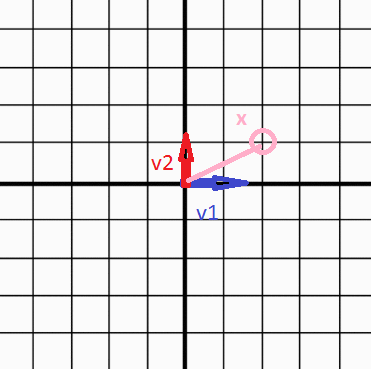
\includegraphics[width=0.3\textwidth]{Standard Basis.png}
\caption {Representing \textbf{x} with standard coordinates. $v_1$ = [1 0]$^T$,$v_2$ = [0 1]$^T$} \textbf{x} = [2 1]$^T$
\end{figure}





\newpage
\section{Here comes the magic}
\subsection{Problem 1}
Let $v_1 = [3/\sqrt(10) \hspace{4mm}1\sqrt(10)]^T
$\newline
Let $v_2 = [1\sqrt(10) \hspace{4mm}-3\sqrt(10)]^T
$

\vspace{4mm}
Show B  = [$v_1$ $v_2$] is an orthonormal basis for $\mathbb{R}^2$

\subsection{Problem 2}
Consider an arbitrary signal of length 2 called \textbf{x}. Multiply this signal by B from Problem 1:

\begin{center}

B\textbf{x} = \textbf{z}

\end{center}

\vspace{10mm}
What matrix times \textbf{z} = \textbf{x}? In other words, solve the following equation for A:

\begin{center}
A\textbf{z} = \textbf{x}

\end{center}

\subsection{Problem 3}
Let \textbf{x} = [2 1]$^T$, from the earlier example\newline
Lets round B to the nearest hundreth, recall $v_1$ and $v_2$ represent coordinate axes:

\begin{center}



\[
B =
\begin{bmatrix}

.95  \hspace{3mm} .32 \\
.32  \hspace{3mm} -.95

\end{bmatrix}
\]

\vspace{3mm}

As a class, draw \textbf{z} onto the new coordinate axis. Figure 1 represented the standard x-y axis, but we can use whatever axis we want.


\begin{figure}[h]
\centering
\includegraphics[width=0.8\textwidth]{NewBasis.png}
\caption {Draw \textbf{x} onto the new coordinate system}
\end{figure}


\end{center}


\newpage


\subsection{Analyze Figure 2}
By looking at the right hand plot of 2.3, determine \textbf{z}.


\vspace{5mm}
\subsection{MAGIC}
Verify your answer from 2.4 by solving for \textbf{z} analytically. Let \textbf{x} = [2 1]$^T$

\vspace{5mm}
\subsection{(more) MAGIC}
What is B$^{-1}$? Hint: use your answer from 2.2

\vspace{4mm}
Verify that:

\begin{center}

B$^{-1}$\textbf{z} = \textbf{x}

\end{center}

\vspace{10mm}
In summary, \textbf{z} and \textbf{x} were not the same, yet they carried the same information. It just depends on what basis was used to represent the signal \textbf{x}


\vspace{5mm}
\section{Inner Product}
Prove the Pythagorean theorem for norms defined by inner products. That is, if z = x + y and \newline
x $\perp$ y, then ||x||$^2$ + ||y||$^2$ = ||z||$^2$




\end{document}